Im ersten Teil soll die Schaltung aus \ref{fig:schalt} ohne den Noise-Verstärker
aufgebaut werden. Für $U_{sig}$ wird eine Frequenz von 420$\si{\hertz}$ und eine
Spannung von $27\si{\milli\volt}$ eingestellt. Die Ausgangssignale werden zu
verschiedenen Phasen skizziert.
\begin{figure}
  \centering
  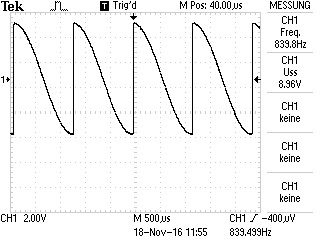
\includegraphics{Bilder/15.jpeg}
  \caption{Phi 15}
  \label{fig:15}
\end{figure}
